\section{Implemented Problems}
\label{sect:ImplementedProblems}
%
%\noindent In this section we give an overview on the implemented problems. At first, we present the strong and weak formulation for the full elliptic PDE and for a standard problem in elasticity. Afterwards, we define spaces for the conforming and non-conforming discretizations. Additionally, we take a look on the mixed formulation with the corresponding spaces.

\noindent The \FFW is able to handle full elliptic problems and problems which arise from elasticity. For these classes of problems conforming, non-conforming and mixed finite element methods are available. In this Section we present the strong and weak formulation of these problems and the corresponding FE-spaces which are implemented. In Table \ref{sect:PDESolver:table:pdeSolver} all available methods are listed. A more detailed mathematical description of the presented problems can be found in \cite{Ar,ArWi,Bra,HaFaIo}.

\medskip

\noindent To get a first impression of the FE-methods, several problems and geometries are already defined in the \FFW\!. The geometry definitions are stored in \path{.\problems\geometries}, whereas the problem definitions for elliptic and elasticity problems are stored in \path{.\problems\elliptic} and \path{.\problems\elasticity}, respectively.

\medskip

\subsection{FEM for Elliptic PDEs}

The general form of an elliptic PDE is given through
\begin{align}\label{sect:FEMForEllipticProblems.eq.strongForm}
-\ddiv(\kappa\cdot\nabla u) + \lambda\cdot\nabla u + \mu u &= f &&\text{in } \Omega, \nonumber\\
u &= u_D &&\text{on } \Gamma_D, \\
\nabla u\cdot\nu &= g &&\text{on } \Gamma_N, \nonumber
\end{align}
with $u_D\in~H^1(\Omega;\R)$, $f\in~L^2(\Omega;\R)$, $g\in~L^2(\Gamma_N;\R)$, $\kappa\in~L^\infty(\Omega;\R^{2\times 2})$, $\lambda\in~L^{\infty}(\Omega,\R^2)$ and $\mu\in~L^\infty(\Omega,\R)$.

\medskip

\noindent The corresponding weak form of \eqref{sect:FEMForEllipticProblems.eq.strongForm} reads: Find $u\in V$ such that
\begin{align}
\label{sect:FEMForEllipticProblems.eq.weakForm}
	\int_\Omega \left( \nabla u\cdot(\kappa\cdot\nabla v) + \lambda\cdot\nabla u\,v + \mu u\,v\right )\,dx = \int_\Omega f\,v\,dx + \int_{\Gamma_N} g\,v\,ds_x.
\end{align}
for all $v\in V$.

\medskip

\noindent To get an approximation of the solution of \eqref{sect:FEMForEllipticProblems.eq.weakForm} several discretization methods are available. One can choose a conforming method where the discrete ansatz-space $V_h$ is a subset of $V$, i.e. $V_h\subset V$, and by that all functions $v_h\in V_h$ are globally continuous. Here one has the choice between the piecewise linear ($P_1$), quadratic ($P_2$) or cubic ($P_3$) FE-ansatz-spaces. Another method which can be taken is the non-conforming Crouzeix-Raviart ($CR$). Here the piecewise linear ansatz-space $V_h$ is not a subset of $V$. Continuity is only enforced on the midpoints of the edges of the underlying triangulation. To get a full detailed description of the theoretical and technical aspects of these methods one may have a look in \cite{Bra}. Here, these standard methods are well introduced. 

\bigskip

\noindent If the main interest is on an accurate stress or flux approximation and some strict equilibration condition rather than the displacement, it might be advantageous to consider an operator split: Instead of one partial differential equation of order $2m$ one considers two equations of order $m$. To be more precise, given one equation in an abstract form $\mathcal{L}u = G$ with some differential operator $\mathcal{L} = \mathcal{A}\mathcal{B}$ composed of $\mathcal{A}$ and $\mathcal{B}$, define $p := \mathcal{B}u$ and solve the two equations $\mathcal{A}p = G$ and $\mathcal{B}u = p$.

\smallskip

\noindent With this splitting, the mixed formulation of \eqref{sect:FEMForEllipticProblems.eq.strongForm} reads: Find $(\sigma,u)\in\Sigma\times V$ such that
\begin{align}\label{sect:FEMForEllipticProblems.eq.mixedStrongForm}
  -\ddiv\sigma + \lambda\cdot(\kappa^{-1}\cdot\sigma) + \mu u &= f &&\text{in } \Omega, \nonumber\\
  \sigma &= \kappa\cdot\nabla u &&\text{in } \Omega,\\
  u &= u_D &&\text{on } \Gamma_D, \nonumber\\
  (\kappa^{-1}\cdot\sigma)\cdot\nu &= g &&\text{on } \Gamma_N\nonumber
\end{align}
with the corresponding weak form
\begin{align}\label{sect:FEMForEllipticProblems.eq.mixedWeakForm}
  \int_\Omega \left( -\ddiv\sigma\,v + \lambda\cdot(\kappa^{-1}\cdot\sigma)\,v + \mu u\,v\right)\,dx &= \int_\Omega f\,v\,dx, \\
  \int_\Omega \left((\kappa^{-1}\cdot\sigma)\cdot\tau + \ddiv\tau\, u\right)\,dx &= \int_{\Gamma_D} u_D(\tau\cdot\nu)\,ds_x,\nonumber
\end{align}
for all $v\in V$ and all $\tau\in\Sigma$.

\bigskip

\noindent In the \FFW the lowest order Raviart-Thomas mixed finite element method ($RT_0-P_0$) of \eqref{sect:FEMForEllipticProblems.eq.mixedWeakForm} is implemented. Here the discrete flux $\sigma_h\in RT_0(\T)\subset H(\ddiv;\Omega)$ is a linear vector field of the form $a\cdot x+b$ with $a\in\R^2$ and $b\in\R$ which is continuous in normal direction. The discrete displacement $u_h\in P_0(\T)\subset L^2(\Omega)$ is piecewise constant. 

\medskip

\noindent An theoretical overview over mixed finite element methods can be found in \cite{Ar,Bra}. The work \cite{BahCC} gives a detailed description of the implemented $RT_0-P_0$ method with focus on the numerical realization.
\bigskip
\subsection{FEM for Elasticity}

\noindent In theory of linear elasticity one is interested in the solution of the following system of elliptic PDE's:
\begin{align}\label{elasticity strong form}
-\ddiv\, \C\,\varepsilon(u)&=f &&\text{in }\Omega,\nonumber\\
u&=u_D &&\text{on }\Gamma_D,\\
(\C\,\varepsilon(u))\cdot \nu&=g &&\text{on }\Gamma_N,\nonumber
\end{align}
with $u_D\in H^1(\Omega;\R^2)$, $f\in L^2(\Omega;\R^2)$, $g\in L^2(\Gamma_N;\R^2)$. Here and throughout, $\varepsilon(v)=\frac{1}{2}(\grad v+(\grad v)^T)$ denotes the linearized Green strain tensor, $\C$ is the reduced symmetric fourth order bounded and positive definite elasticity tensor defined by the Lam\'e parameters $\lambda$ and $\mu$. In Voigt notation the tensor $\C$ and its inverse is given through
\begin{equation*}
\C:=\begin{pmatrix}
2\mu+\lambda & \lambda       & 0\\
\lambda      & 2\mu+\lambda  & 0\\
0            & 0             & \mu
\end{pmatrix} \quad\text{and}\quad
\Cinv:=\begin{pmatrix}
\frac{\lambda+2 \mu}{4\mu(\lambda+\mu)} & \frac{-\lambda}{4\mu(\lambda+\mu)}            & 0\\
\frac{-\lambda}{4\mu(\lambda+\mu)}          & \frac{\lambda+2 \mu}{4\mu(\lambda+\mu)} & 0\\
0 & 0 & \frac{1}{\mu}
\end{pmatrix}.
\end{equation*}

\noindent There are several formulations of the problem \eqref{elasticity strong form} depending on the focus of interest. For instant, \eqref{elasticity strong form} is a displacement based formulation. Here, one computes an approximation of the displacement $u$ and afterwards the discrete solution $u_h$ is post-processed to get the discrete strain and stress of the problem. In other formulations strain or stress are computed directly. The \FFW offers a displacement-based and a stress-displacement-based formulation. Both can be found in \cite{Bra}.

\bigskip

\noindent Similar to the elliptic problems, there are conforming and nonconforming FE-methods which one can choose to solve \eqref{elasticity strong form}. At first, the weak formulation is given: Seek $u\in V$ such that
\begin{equation}\label{elasticity weak form}
\int_{\Omega} \varepsilon(u):\C\varepsilon(v) \, dx = \int_{\Omega}
f \cdot v \, dx + \int_{\Gamma_N} g\cdot v \, ds_x \quad\text{for
all } v \in V.
\end{equation}

\noindent The conforming $P_1-P_1$ FE-method approximates the displacement $u\in H^1(\Omega)^2$ in each component with the linear ansatz space $P_1$. Since this kind of approximations does not work for incompressible materials like rubber or water, the so-called locking effect, there is also a nonconforming method available. The Kouhia-Stenberg element ($P_1-CR$) approximates the first component of $u$ with the globally continuous piecewise linear ansatz-space ($P_1$) and the second one with the Crouzeix-Raviart ansatz-space ($CR$). The Kouhia-Stenberg element is able to handle also incompressible materials. Details can be found in \cite{Bra,KoSt}. Problems will arise in the condition number of the energy matrix for incompressible materials. To get rid of it one has to change the problem formulation. A stress-displacement formulation which results in a mixed scheme handles then both problems: the locking effect and the dependence of the condition number for incompressible materials. This formulation and the FE-spaces we will describe as next.

\bigskip

%\noindent If the main interest is on an accurate stress or flux approximation and some strict equilibration
%condition rather than the displacement, it might be advantageous to consider an operator split: Instead of
%one partial differential equation of order $2m$ one considers two equations of order $m$.
%To be more precise, given one equation in an abstract form $\mathcal{L}u = G$ with some differential
%operator $\mathcal{L} = \mathcal{A}\mathcal{B}$ composed of $\mathcal{A}$ and $\mathcal{B}$, define $p := \mathcal{B}u$ and solve the two equations
%$\mathcal{A}p = G$ and $\mathcal{B}u = p$.\smallskip\\
%\noindent
%The mixed form of \eqref{elasticity strong form} reads:

\noindent The stress-displacement formulation of \eqref{elasticity strong form} is given through: Seek $(\sigma,u)\in\Sigma\times V$ such that
\begin{align}\label{elasticity mixed strong form}
		-\ddiv\, \sigma&=f&  &\text{ and }& \sigma&=\C\,\varepsilon(u)&\text{  in }\Omega,\\
		u&=u_D\text{ on }\Gamma_D& &\text{ and }& \sigma \nu&=g \text{ on }\Gamma_N.\nonumber
\end{align}
Then, the corresponding weak form reads
\begin{align*}
\int_{\Omega} \sigma:\C^{-1}\tau \, dx + \int_{\Omega} u\cdot\ddiv\,
\tau \,dx
&= \int_{\Gamma_D} u_D\cdot (\tau \,\nu) \, ds_x &&\text{for all } \tau \in \Sigma,\\
\int_{\Omega} v\cdot\ddiv\, \sigma\,dx &= - \int_{\Omega} f \cdot v
\, dx &&\text{for all } v \in V.
\end{align*}

\noindent One way to handle \eqref{elasticity mixed strong form} is the Peers-element which is described in \cite{CCDo}. The problem with that element is symmetry of the stress $\sigma$. This is only enforced weakly with a side constraint. In the \FFW we have implemented another mixed finite element based on the work of Arnold and Winther \cite{ArWi}. They have introduced a mixed finite element of problem \eqref{elasticity mixed strong form} which is locking-free (with a condition number which is independent of the current material) and the discrete stress $\sigma_h$ is symmetric in a natural way. Details on the implementation can be found in \cite{CCGuReTh}.

\bigskip
\subsection{Predefined Problem Definitions}
\label{sect:ImplementedProblems_ProblemDefinition}

\noindent There are various problem definitions for elliptic PDEs and for linear elasticity already defined, for which we give an overview in the following.

\medskip

\noindent All problem definitions contain functions for the coefficients $\kappa$, $\lambda$, $\mu$, the external load $f$, and the boundary $u_D$ and $g$. Some of the problem-definition-filenames contain a suffix \path{_exact}. Here a function $u_{\text{exact}}$ which represents the exact solution is given and the data-functions $f$, $u_D$ and $g$ are computed automatically. With those problem definitions it is possible to compute the exact errors, e.g. energy error between $u_h$ and $u_{\text{exact}}$. Problem definitions for elasticity additionally contain standard parameters for the material parameter $\nu$ and $E$.

\bigskip

\noindent If you want to create your own problem definition, create an \code{.m}-file named \path{Elliptic_<problemName>} in \path{.\problems\elliptic} or \path{Elasticity_<problemName>} in (\path{.\problems\elasticity}), which contains all necessary information. For details concerning the structure of the problem definition, see Section \ref{sect:QuickStart}.

\bigskip

\subsubsection{Predefined Problem Definitions for Elliptic PDEs}$ $\\

\noindent\emph{Elliptic\_Lshape}

\smallskip

\noindent Model example $-\Delta u = 1$, $u_D=0$ and $g=0$ on an L-shaped domain.

\bigskip

\noindent\emph{Elliptic\_Lshape\_exact}

\smallskip

\noindent The exact solution $u(r,\phi)=r^{2/3}\sin(2/3\phi)$ in polar coordinates on an L-shaped domain with Neumann boundary is given. The corresponding right hand side $f$ is zero and induced boundary data. The coefficients of the elliptic PDE correspond to the Laplacian operator.
\bigskip

\noindent\emph{Elliptic\_Square}\smallskip\\
Model example $-\Delta u = 1$, $u_D=0$ and $g=0$ on a squared domain.
\bigskip

\noindent\emph{Elliptic\_Square\_exact}\smallskip\\
The exact solution $u(x,y) = x(1-x)\,y(1-y)$ as well as its gradient and the right-hand side $f$ are given with the PDE-coefficients $\kappa$, $\lambda$ and $\mu$ all zero, on a squared domain is given.
\bigskip

\noindent\emph{Elliptic\_SquareFullElliptic\_exact}\smallskip\\
The exact solution $u(x,y) = \sin(x^3)\cos(y^\pi)+x^8-y^9+x^6 y^{10}$ with the PDE-coefficients $\kappa$ being the identity, $\lambda = \left( \begin{smallmatrix} 5\sin(x+y)\\ 6\cos(x+y) \end{smallmatrix}\right)$ and $\mu=7$ on a squared domain is given. The symbolic toolbox of MATLAB computes all necessary information, i.e., $f$, $u_D$ and $g$.
\bigskip

\noindent\emph{Elliptic\_HexagonalSlit\_exact}\smallskip\\
The exact solution $u(r,\phi)=r^{1/4}\sin(1/4\phi)$ in polar coordinates with the load $f\equiv0$, the Dirichlet function $u_D=u|_{\Gamma_D}$, and coefficients belonging to the Laplacian are given on a slitted hexagon.
\bigskip

\noindent\emph{Elliptic\_Waterfall\_exact}\smallskip\\
The waterfall function $$u(x,y) = xy(1-x)(1-y) \arctan\left(k(\sqrt{(x-5/4)^2 + (y+1/4)^2}-1)\right)$$ is given. The parameter $k$ controls the slope of $u$. For $k\rightarrow\infty$ the slope of the function tends to infinity. This parameter is stored in the structure \code{p} at \code{p.PDE.k} and can be changed in the starting scripts. The domain is a square with homogeneous Dirichlet boundary. We look at the problem $-\Delta u = f$. The load $f$ is computed from $u$.
\bigskip

\noindent\emph{Elliptic\_Template}\smallskip\\
A predefined template for generating problem definitions. For given data $f, u_D$ and $g$ one can compute the corresponding discrete solution $u_h$.
\bigskip

\noindent\emph{Elliptic\_Template\_Exact}\smallskip\\
A predefined template for generating problem definitions. For a given function $u_{\text{exact}}(x,y)$ in cartesian coordinates and coefficients $\kappa,\lambda,\mu$, the symbolic toolbox of MATLAB computes all necessary information, i.e., $f$, $u_D$ and $g$.
\bigskip


\subsubsection{Predefined Problem Definitions for Elasticity}$ $\\

\noindent\emph{Elasticity\_Cooks}\smallskip\\
A tapered panel is clamped on one end and subjected to a surface load in
vertical direction on the opposite end with $f = 0$ and $g(x, y) = (0, 1000)$ if
$(x, y) \in  \Gamma_N$ with $x = 48$ and $g = 0$ on the remaining part of $\Gamma_N$, the Young modulo $E =
2900$, and the Possion ratio $\nu = 0.3$.
\bigskip


\noindent\emph{Elasticity\_Square\_exact}\smallskip\\
The unit square with the given function $u(x,y)=10^{-5}\left(\begin{smallmatrix} \cos((x+1)(y+1)^2) \\
\sin((x+1))\cos(y+1) \end{smallmatrix}\right)$. Young modulo and the Possion ratio are set to $E=10^5$ and $\nu = 0.3$.
\bigskip


\noindent\emph{Elasticity\_Square\_Neumann\_exact}\smallskip\\
Besides the geometry we have the same problem definition as in \emph{Elasticity\_Square}. The domain changes from \code{Square} to \code{SquareNeumann}.
\bigskip


\noindent\emph{Elasticity\_Lshape\_exact}\smallskip\\
Using polar coordinates $(r, \theta)$, $-\pi < \theta \leq \pi$ $u$ with radial component $u_r,u_\theta$ reads
$$
u_{r}(r,\theta) = \frac{r^{\alpha}}{2\mu}
    (-(\alpha+1)\cos((\alpha+1)\theta)+
           \nonumber     (C_{2}-
    (\alpha+1))C_{1}\cos((\alpha-1)\theta)),
$$
and
$$ u_{\theta}(r,\theta) = \frac{r^{\alpha}}{2\mu}
    ((\alpha+1)\sin((\alpha+1)\theta)+
          \nonumber     (C_{2}+\alpha-1)C_{1}\sin((\alpha-1)\theta)).
$$
The parameters are
$C_{1}=-\cos((\alpha+1)\omega)/\cos((\alpha-1)\omega)$, $C_{2} = 2(\lambda+2\mu)/(\lambda+\mu)$ where $\alpha = 0.54448...$ is the positive solution of  $\alpha \sin 2\omega + \sin 2\omega\alpha = 0$ for $ \omega= 3 \pi /4$; the Young modulus is $E=10^5$, Poisson ratio $\nu = 0.3$, and the volume force $f\equiv 0$.
\bigskip


\noindent\emph{Elasticity\_Template}\smallskip\\
A predefined template for generating problem definitions. For given data $f,u_D$ and $g$ and coefficients $\kappa,\lambda,\mu$ one can compute the corresponding discrete solution $u_h$.
\bigskip


\noindent\emph{Elasticity\_Exact\_Template}\smallskip\\
A predefined template for generating problem definitions. For a given function $u_{\text{exact}}(x,y)$ in cartesian coordinates, the symbolic toolbox of MATLAB computes all necessary information, i.e., $f$, $u_D$ and $g$. 
\subsection{Geometries}
\label{sect:ImplementedProblems_Geometries}

In the following we give an overview about the geometries which are already available. For adding a new geometry create a new directory \code{<newGeometry>} in \path{./problems/geometries/}. There you have to define the coordinates of the geometry in \path{<newGeometry>_c4n.dat}. The nodes for each triangle have to be defined in \path{<newGeometry>_n4e.dat}. The Dirichlet- and Neumann-part of the domain boundary is specified in \path{<newGeometry>_Db.dat} and \path{<newGeometry>_Nb.dat} respectively.

\begin{figure}[h!]
\includegraphics[width=0.15\textwidth]{images/sect_ImplementedProblems_Triangle.pdf}
\includegraphics[width=0.15\textwidth]{images/sect_ImplementedProblems_Square.pdf}
\includegraphics[width=0.15\textwidth]{images/sect_ImplementedProblems_Lshape.pdf}
\includegraphics[width=0.15\textwidth]{images/sect_ImplementedProblems_Lshape3.pdf}
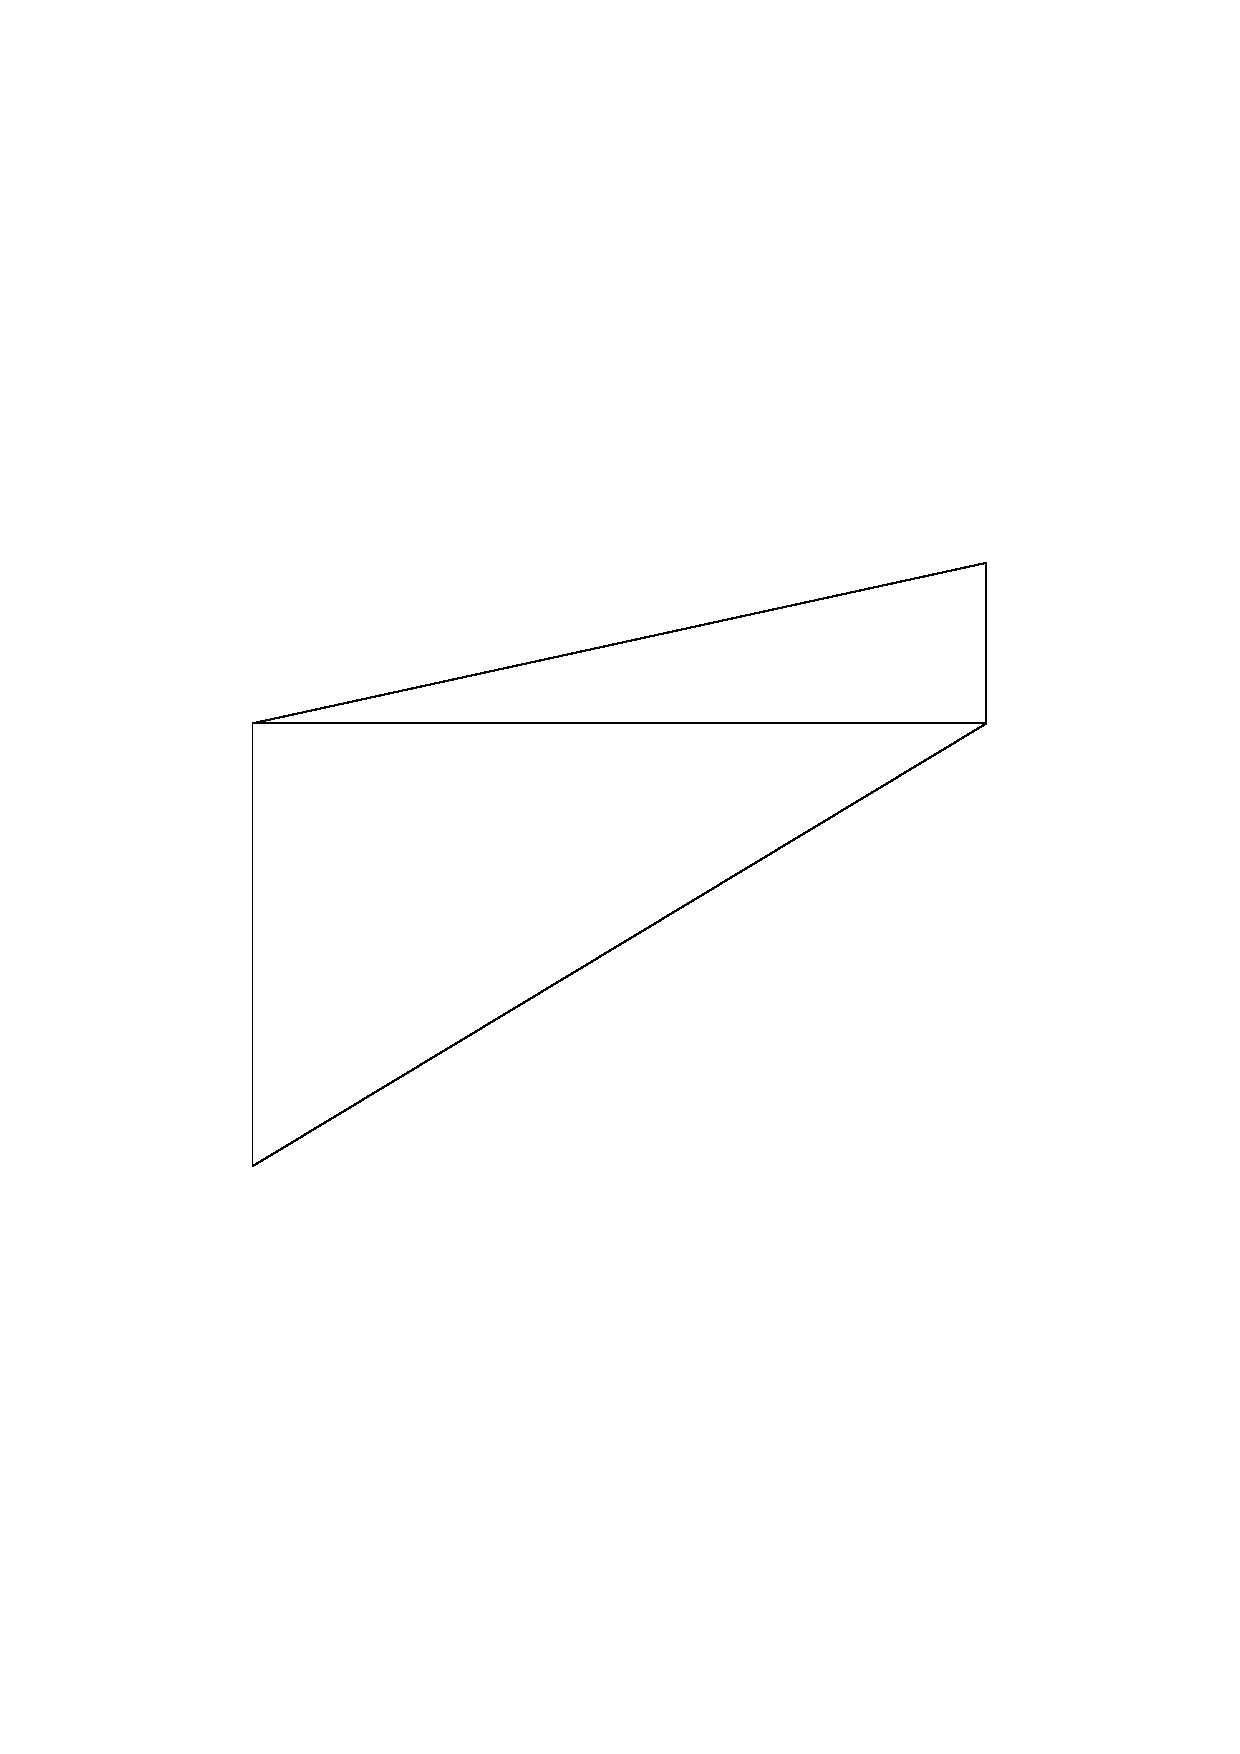
\includegraphics[width=0.15\textwidth]{images/sect_ImplementedProblems_Cooks.pdf}
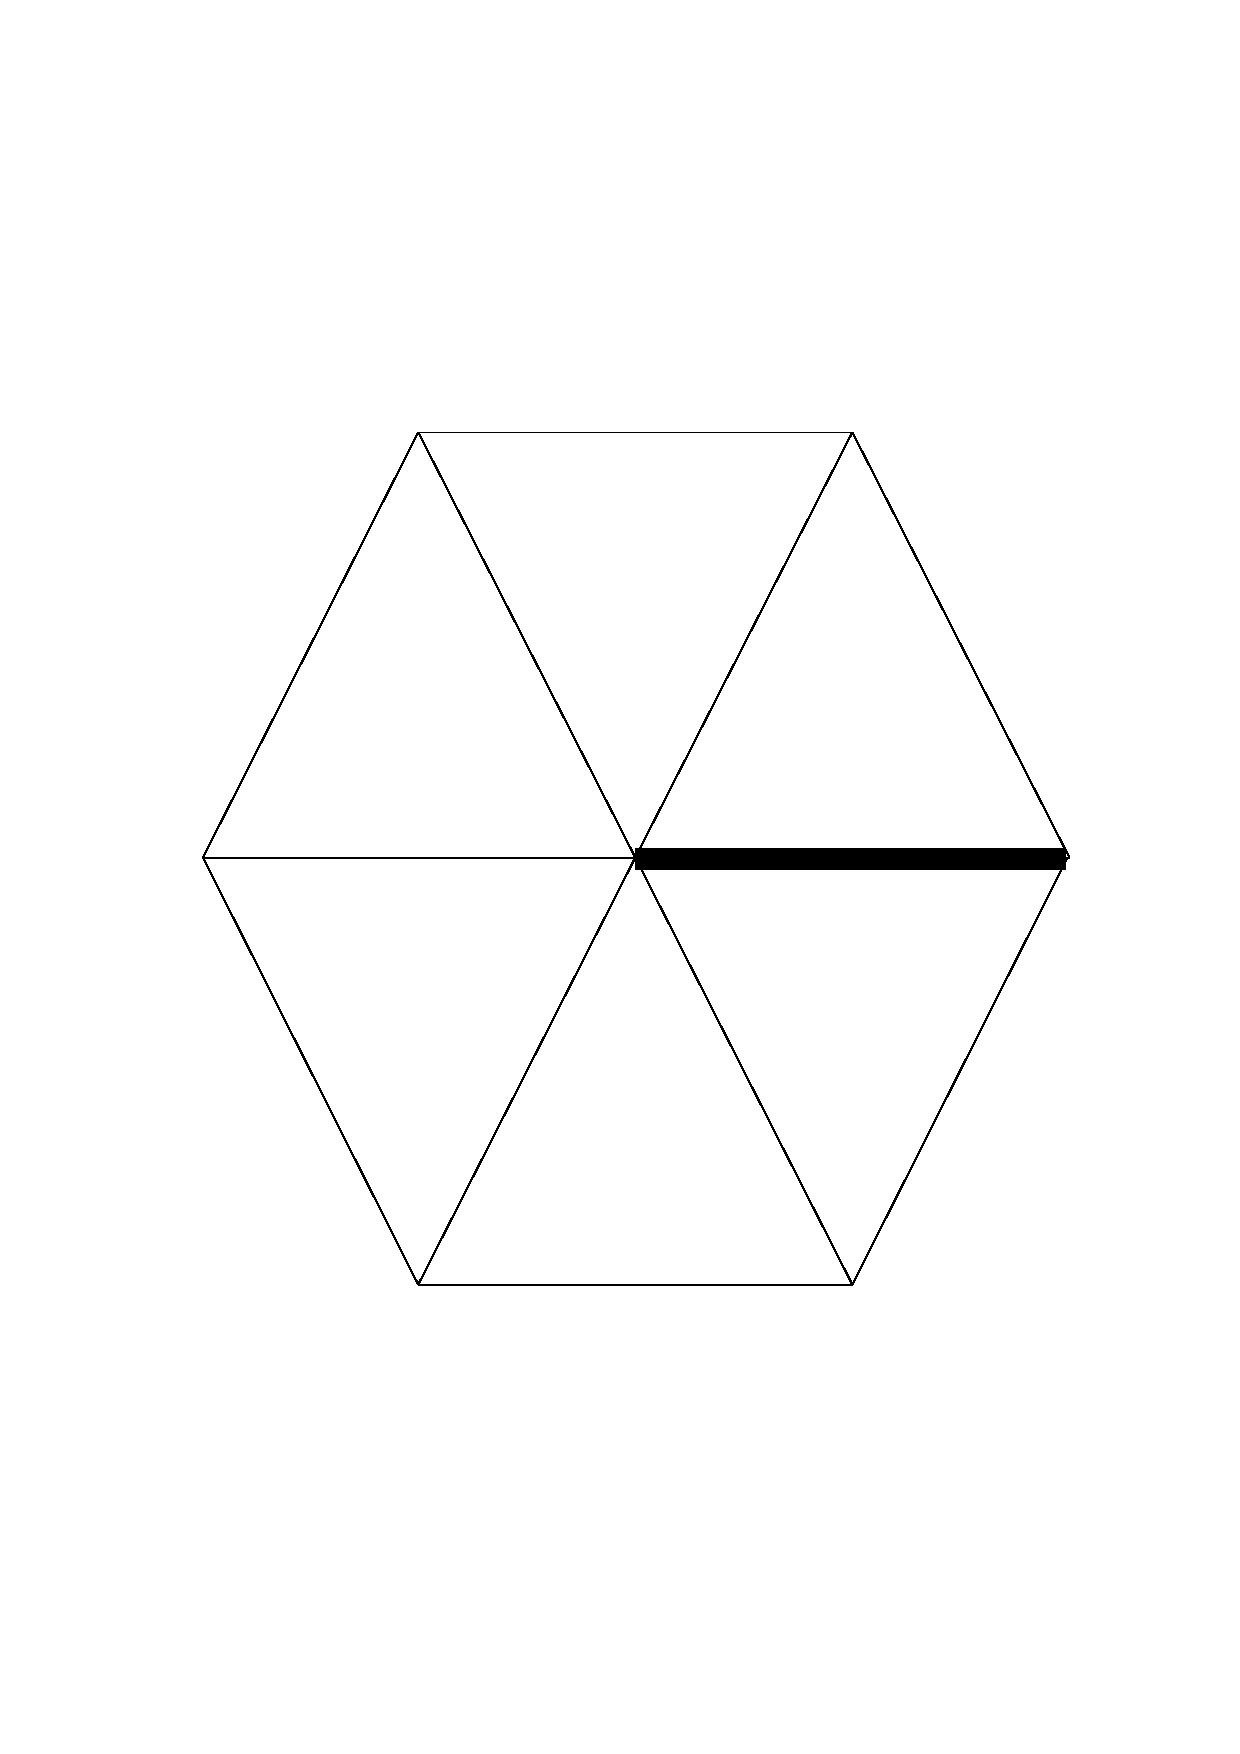
\includegraphics[width=0.15\textwidth]{images/sect_ImplementedProblems_HexagonalSlit.pdf}
\caption{Initial triangulation of implemented geometries. From left to right: Triangle, Square, Lshape, Lshape3, Cooks, HexagonalSlit}
\end{figure}

\begin{tabular}{p{0.25\textwidth}p{0.65\textwidth}}
Geometry Name 	& 	Description \\
\hline
Triangle				& The reference triangle $\Omega=\conv\{(0,0),(1,0),(0,1)\}$ with pure Dirichlet-boundary.\\
Square					& The unit square $\Omega=[0,1]^2$ with pure Dirichlet-boundary.\\
SquareNeumann		& The unit square with Neumann boundary $\Gamma_N=\conv\{(1,0),(1,1)\}$.\\
Lshape          & The L-shaped domain $\Omega=[-1,1]^2\setminus\{(0,1]\times(0,-1]\}$ with pure Dirichlet-boundary.\\
LshapeNeumann		& The domain is the L-shape domain with Neumann boundary.  $\Gamma_D=\left\{\conv\{(0,0),(1,0)\}\cup\conv\{(0,0),(0,-1)\}\right\}$.\\
Lshape3         & Lshape3 is a rotated version of Lshape. Here the boundary of the rotated L-shaped domain is not axis parallel anymore.\\
Lshape3Neumann  & Lshape3Neumann is a rotated version of LshapeNeumann.\\
Cooks						& Geometry for the Cook's membrane problem in elasticity. $\Omega=\conv\{(0,0),(48,44),(48,60),(0,44)\}$. The Dirichlet boundary $\Gamma_D$ is $\conv\{(0,0),(0,44)\}$. Thus the Neumann boundary is $\partial\Omega\setminus\Gamma_D$.\\
HexagonalSlit   & We have defined a hexagon $\Omega\subset[-1,1]^2$ which is slitted in $\{0\}\times[0,1]$. The slit is approximated by adding an additional node through a small, numerically insignificant, perturbation of the node $(0,1)$. The slitted hexagon is an example for a non-Lipschitz domain with pure Dirichlet boundary.
\end{tabular}

%\subsection{Eigenwert Probleme}
Gesucht sind die Eigenwerte $\omega$ und Eigenfunktionen $u$, $\lVert u\rVert_{L^2}=1 $, des elliptischen Eigenwertproblems
\begin{align*}
  -div(\kappa(x)\cdot\nabla u) + \lambda(x)\cdot\nabla u + \mu(x)\cdot u &= \omega u \\
\nonumber
  u &= u_D \hbox{, auf } \Gamma_D \\
  \frac{\partial u}{\partial \eta} &= g \hbox{, auf } \Gamma_N\; .
\end{align*}
Damit das \FFW alle Einstellungen in Bezug auf Eigenwertprobleme
�bernimmt muss zuerst
\begin{verbatim}
p.params.problem.type = 'eigenvalue';
p.params.solver = 'eigenvalue';
\end{verbatim}
gesetzt werden. Dies kann auch mittels eines Aufrufs von
\begin{verbatim}
p = configureP(pdeSolver,problem,mark,maxNrDoF,[],'eigenvalue');
\end{verbatim}
geschehen.\\
In der Datei \path{startEigenvalue.m} wurden alle Einstellungen schon vorgenommen. Dort stehen auch ein paar Problemstellungen zur Auswahl.

\subsubsection{Lineares Gleichungssystem l�sen}
\hspace{0cm}

\medskip
\noindent
\textbf{Datei:} \path{algorithms/linSysSolvers/eigenvalue/solve.m}\\[1.5ex]
Durch Finite Element Discretisierung des Eigenwert Problems erh�lt man ein verallgemeinertes Eigenwertproblem f�r Matrizen.
\begin{equation*}
A u = \omega B u\;
\end{equation*}
Es wird die Funktion \code{eigs} von MATLAB benutzt die unter Anderem auf das Packet ARPACK zur�ckgreift. Der Parameter \code{p.params.curEigenvalue} gibt dabei an, welcher Eigenwert berechnet werden soll. \code{eigs} berechnet alle \code{curEigenvalue} kleinsten Eigenwerte und Eigenfunktionen. Da das Gitter aber nur f�r den einen Eigenwert bzw. Eigenfunktion adaptiv verfeinert werden kann, wird auch nur dieser gespeichert. Die Anzeige wird vorher auf 'stumm' gestellt.
\begin{verbatim}
options.disp = 0;
[V,D] = eigs(A(freeNodes,freeNodes),B(freeNodes,freeNodes),...
             curEigenvalue,'sm',options);
\end{verbatim}

\subsubsection{PDESolver}
Zur Zeit ist nur die P1-FEM implementiert. Diese befindet sich im Ordner \path{/PDESolvers/P1-Eigenvalue}.
\begin{verbatim}
p.params.pdeSolver = 'P1-Eigenvalue';
\end{verbatim}
Die Steifigkeitsmatrix A und die Massenmatrix B wird dabei in
\begin{verbatim}
p.level(end).A
p.level(end).B
\end{verbatim}
gespeichert.

\subsubsection{Problem}
Zwei Problemdefinitionen stehen aktuell zur Verf�gung. Zum einen das Laplace Problem auf dem Quadrat f�r homogene Randdaten und zum anderen das Laplace Problem auf dem L-Shape ebenfalls mit homogenen Randdaten. Diese befinden sich im Verzeichniss \path{/problems/eigenvalue/}
\begin{verbatim}
p.params.problem.name = 'Laplace-Square-exact';
p.params.problem.name = 'Laplace-Lshape';
\end{verbatim}

\subsubsection{Parameter}
\hspace{0cm}

\medskip \noindent
\textbf{p.params.curEigenvalue}\\
Gibt an welcher Eigenwert ausgehend vom kleinsten Eigenwert berechnet werden soll (Default = 1).

\medskip \noindent
\textbf{p.params.modules.mark.refineFirstLevel}\\
Um gr�ssere Eigenwerte berechnen zu k�nnen muss auch die Matrix gross genug sein. D.h. es m�ssen gen�gend innere Knoten vorhanden sein. Um das zu garantieren kann mit diesem Parameter angegeben werden wie oft das Gitter uniform verfeinert wird, bevor die erste L�sung berechnet wird (Default = 1).

\subsubsection{ErrorType}
Zus�tzlich zu den anderen Typen ('estimatedError', 'L2error', 'H1semiError') steht bei Eigenwert Problemen noch der Typ 'eigenvalueError' zur Verf�gung. So l�sst sich mittels
\begin{verbatim}
p = show('drawError_eigenvalueError',p);
\end{verbatim}
der exakte Fehler des Eigenwertes in einer Graphik mit logarithmischen Skalen darstellen. Dazu mus vorher der exakte Eigenwert definiert worden sein.
\begin{verbatim}
p.problem.eigenvalue_exact = exakter Eigenwert;
\end{verbatim}

